%封面摘要部分
\newcommand{\coverabstract}{
    \begin{large}
        猫,属于猫科动物,分家猫、野猫,是全世界家庭中较为广泛的宠物。家猫的祖先据推测是古埃及的沙漠猫,
        波斯的波斯猫,已经被人类驯化了3500年(但未像狗一样完全地被驯化)。一般的猫:头圆、颜面部短,
        前肢五指,后肢四趾,趾端具锐利而弯曲的爪,爪能伸缩。夜行性。以伏击的方式猎捕其它动物,大多能攀援上树
        猫的趾底有脂肪质肉垫,以免在行走时发出声响,捕猎时也不会惊跑鼠。行进时爪子处于收缩状态,防止爪被磨钝,
        在捕鼠和攀岩时会伸出来
    \end{large}
    \newline
    \newline\\
    \newline\\
    \newline
    \begin{figure}[H]
        \begin{center}
            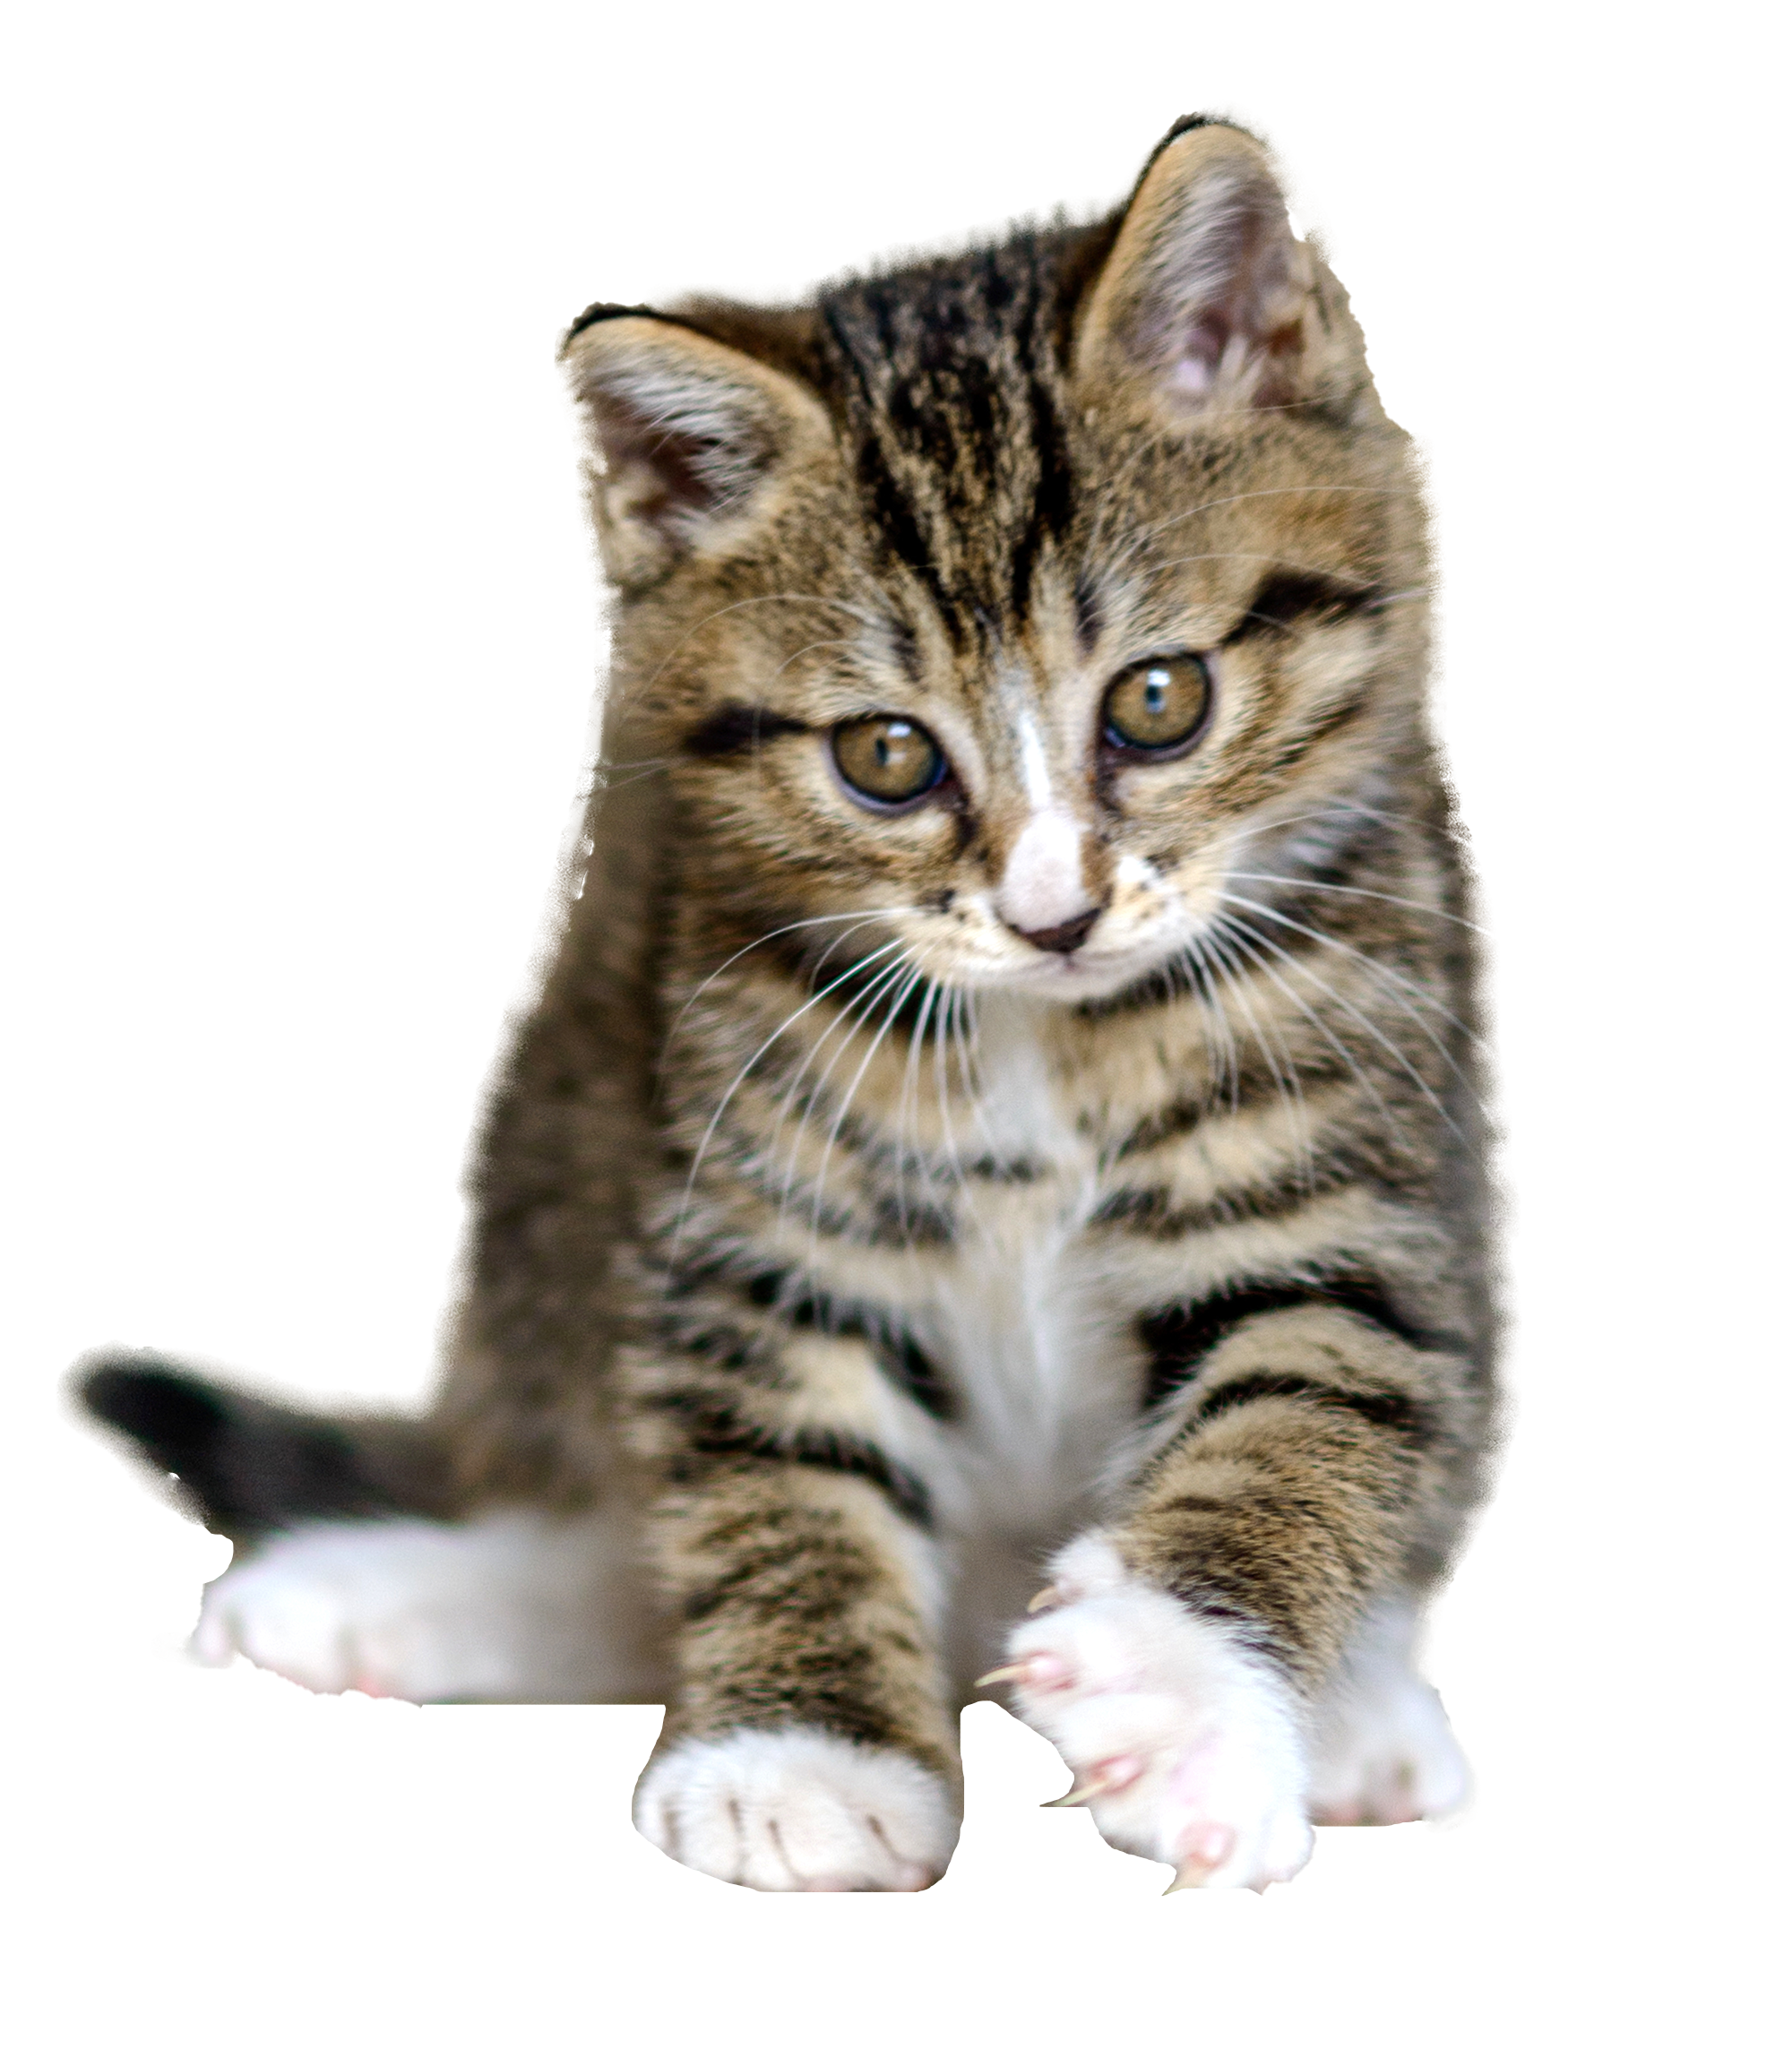
\includegraphics[width=0.7\linewidth]{Figures/images/cat}
        \end{center}
        \begin{center}
             \qquad \qquad 图1
        \end{center}
        \label{fig:tstmp20211203103404}
    \end{figure}
    
}

